\documentclass[a4paper, fleqn]{article}
\usepackage[utf8]{inputenc}
\usepackage{amsmath}
\usepackage{amssymb}
\usepackage{caption}
\usepackage{mathtools}
\usepackage{amsfonts}
\usepackage{lastpage}
\usepackage{tikz}
\usepackage{float}
\usepackage{textcomp}
\usetikzlibrary{patterns}
\usepackage{pdfpages}
\usepackage{gauss}
\usepackage{fancyvrb}
\usepackage[table]{colortbl}
\usepackage{fancyhdr}
\usepackage{graphicx}
\usepackage[margin=2.5 cm]{geometry}

\setlength\parindent{0pt}
\setlength\mathindent{75pt}

\definecolor{listinggray}{gray}{0.9}
\usepackage{listings}
\lstset{
	language=,
	literate=
		{æ}{{\ae}}1
		{ø}{{\o}}1
		{å}{{\aa}}1
		{Æ}{{\AE}}1
		{Ø}{{\O}}1
		{Å}{{\AA}}1,
	backgroundcolor=\color{listinggray},
	tabsize=3,
	rulecolor=,
	basicstyle=\scriptsize,
	upquote=true,
	aboveskip={0.2\baselineskip},
	columns=fixed,
	showstringspaces=false,
	extendedchars=true,
	breaklines=true,
	prebreak =\raisebox{0ex}[0ex][0ex]{\ensuremath{\hookleftarrow}},
	frame=single,
	showtabs=false,
	showspaces=false,
	showlines=true,
	showstringspaces=false,
	identifierstyle=\ttfamily,
	keywordstyle=\color[rgb]{0,0,1},
	commentstyle=\color[rgb]{0.133,0.545,0.133},
	stringstyle=\color[rgb]{0.627,0.126,0.941},
  moredelim=**[is][\color{blue}]{@}{@},
}

\lstdefinestyle{base}{
  emptylines=1,
  breaklines=true,
  basicstyle=\ttfamily\color{black},
}

\pagestyle{fancy}
\def\checkmark{\tikz\fill[scale=0.4](0,.35) -- (.25,0) -- (1,.7) -- (.25,.15) -- cycle;}
\newcommand*\circled[1]{\tikz[baseline=(char.base)]{
            \node[shape=circle,draw,inner sep=2pt] (char) {#1};}}
\newcommand*\squared[1]{%
  \tikz[baseline=(R.base)]\node[draw,rectangle,inner sep=0.5pt](R) {#1};\!}
\newcommand{\comment}[1]{%
  \text{\phantom{(#1)}} \tag{#1}}
\def\el{[\![}
\def\er{]\!]}
\def\dpip{|\!|}
\def\MeanN{\frac{1}{N}\sum^N_{n=1}}
\cfoot{Page \thepage\ of \pageref{LastPage}}
\DeclareGraphicsExtensions{.pdf,.png,.jpg}

\author{Nikolaj Dybdahl Rathcke (Student ID: 74763954)}
\title{Relational Methods \\ Assignment 1}
\lhead{Relational Methods}
\rhead{Assignment 1}

\begin{document}
\maketitle

\section{Specific Relations}
\subsection{(a)}
Say we have the following two relations $R$ and $S$ on $A=\{1,2\}$:
\begin{align*}
  R&=
  \begin{pmatrix}
    1 & 1 \\
    0 & 1
  \end{pmatrix}
  \ \ \ \ \
  S=
  \begin{pmatrix}
    0 & 0 \\
    0 & 1
  \end{pmatrix}
\end{align*}
Then we have
\begin{align*}
  (RS)^T&=
  \begin{pmatrix}
    0 & 0 \\
    1 & 1
  \end{pmatrix}
  \ \ \ \ \
  R^TS^T=
  \begin{pmatrix}
    0 & 0 \\
    0 & 1
  \end{pmatrix}
\end{align*}
so they are not the same.

\subsection{(b)}
We start by calculating $\overline{R}$ and its transpose:
\begin{align*}
  \overline{R} &=
  \begin{pmatrix}
    1 & 0 & 0 & 1 \\
    0 & 1 & 0 & 0 \\
    1 & 0 & 1 & 1 \\
    1 & 0 & 0 & 0
  \end{pmatrix}
  \ \ \ \ \
  \overline{R}^T
  \begin{pmatrix}
    1 & 0 & 1 & 1 \\
    0 & 1 & 0 & 0 \\
    0 & 0 & 1 & 0 \\
    1 & 0 & 1 & 0
  \end{pmatrix}
\end{align*}
So we have the intersection is:
\begin{align*}
  \left( \overline{R}^T\cap R\right) =
  \begin{pmatrix}
    1 & 0 & 1 & 1 \\
    0 & 1 & 0 & 0 \\
    0 & 0 & 1 & 0 \\
    1 & 0 & 1 & 0
  \end{pmatrix} \cap
  \begin{pmatrix}
    0 & 1 & 1 & 0 \\
    1 & 0 & 1 & 1 \\
    0 & 1 & 0 & 0 \\
    0 & 1 & 1 & 1
  \end{pmatrix} =
 \begin{pmatrix}
    0 & 0 & 1 & 0 \\
    0 & 0 & 0 & 0 \\
    0 & 0 & 0 & 0 \\
    0 & 0 & 1 & 0
  \end{pmatrix}
\end{align*}
Multiplying it by $R$ gives us:
\begin{align*}
  \left( \overline{R}^T\cap R\right) R =
 \begin{pmatrix}
    0 & 0 & 1 & 0 \\
    0 & 0 & 0 & 0 \\
    0 & 0 & 0 & 0 \\
    0 & 0 & 1 & 0
  \end{pmatrix}
  \begin{pmatrix}
    0 & 1 & 1 & 0 \\
    1 & 0 & 1 & 1 \\
    0 & 1 & 0 & 0 \\
    0 & 1 & 1 & 1
  \end{pmatrix} =
  \begin{pmatrix}
    0 & 1 & 0 & 0 \\
    0 & 0 & 0 & 0 \\
    0 & 0 & 0 & 0 \\
    0 & 1 & 0 & 0
  \end{pmatrix}
\end{align*}
Unioned with $\overline{R}$ gives us:
\begin{align*}
  \left( \overline{R}^T\cap R\right) R\cup \overline{R} =
 \begin{pmatrix}
    0 & 1 & 0 & 0 \\
    0 & 0 & 0 & 0 \\
    0 & 0 & 0 & 0 \\
    0 & 1 & 0 & 0
  \end{pmatrix} \cup
  \begin{pmatrix}
    1 & 0 & 0 & 1 \\
    0 & 1 & 0 & 0 \\
    1 & 0 & 1 & 1 \\
    1 & 0 & 0 & 0
  \end{pmatrix} =
  \begin{pmatrix}
    1 & 1 & 0 & 1 \\
    0 & 1 & 0 & 0 \\
    1 & 0 & 1 & 1 \\
    1 & 1 & 0 & 0
  \end{pmatrix}
\end{align*}
To find The reflexive closure, we need to add $1$'s on the diagonal (so every
element is related to itself), so we need to add $(4,4)$. To find the transitive closure, lets look at graph to see
what entries we need:
\begin{figure}[H]
  \centering
  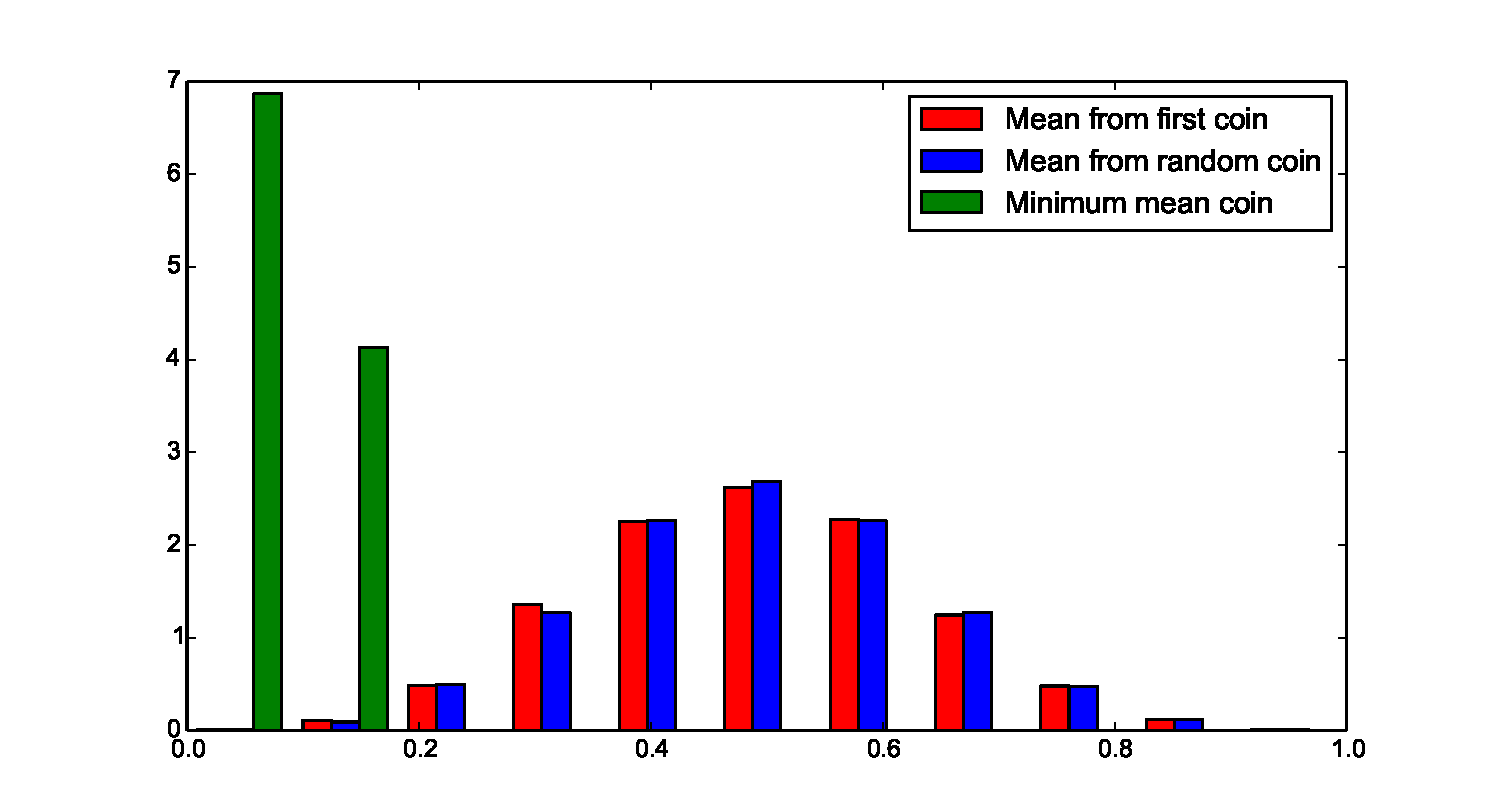
\includegraphics[scale=0.5]{fig2}
  \caption{Graph given by the relation above.}
  \label{fig2}
\end{figure}
So we can reach $1$, $2$ and $4$ from $1$. We can only reach $2$ from $2$. We can get to
any element from $3$ and we can reach $1$, $2$ and $4$ from $4$. \\
This means we need to add $(3,2)$ and $(4,4)$ giving us:
\begin{align*}
  \left(\left( \overline{R}^T\cap R\right) R\cup \overline{R}\right)^*  =
  \begin{pmatrix}
    1 & 1 & 0 & 1 \\
    0 & 1 & 0 & 0 \\
    1 & 1 & 1 & 1 \\
    1 & 1 & 0 & 1
  \end{pmatrix}
\end{align*}
which is the reflexive-transitive closure of the relation above.

\subsection{(c)}
To get the reflexive closure of $R$, we just need to calculate $R\cup I$. To get the
transitive closure, lets look at the graph given by the relation $R$:
\begin{figure}[H]
  \centering
  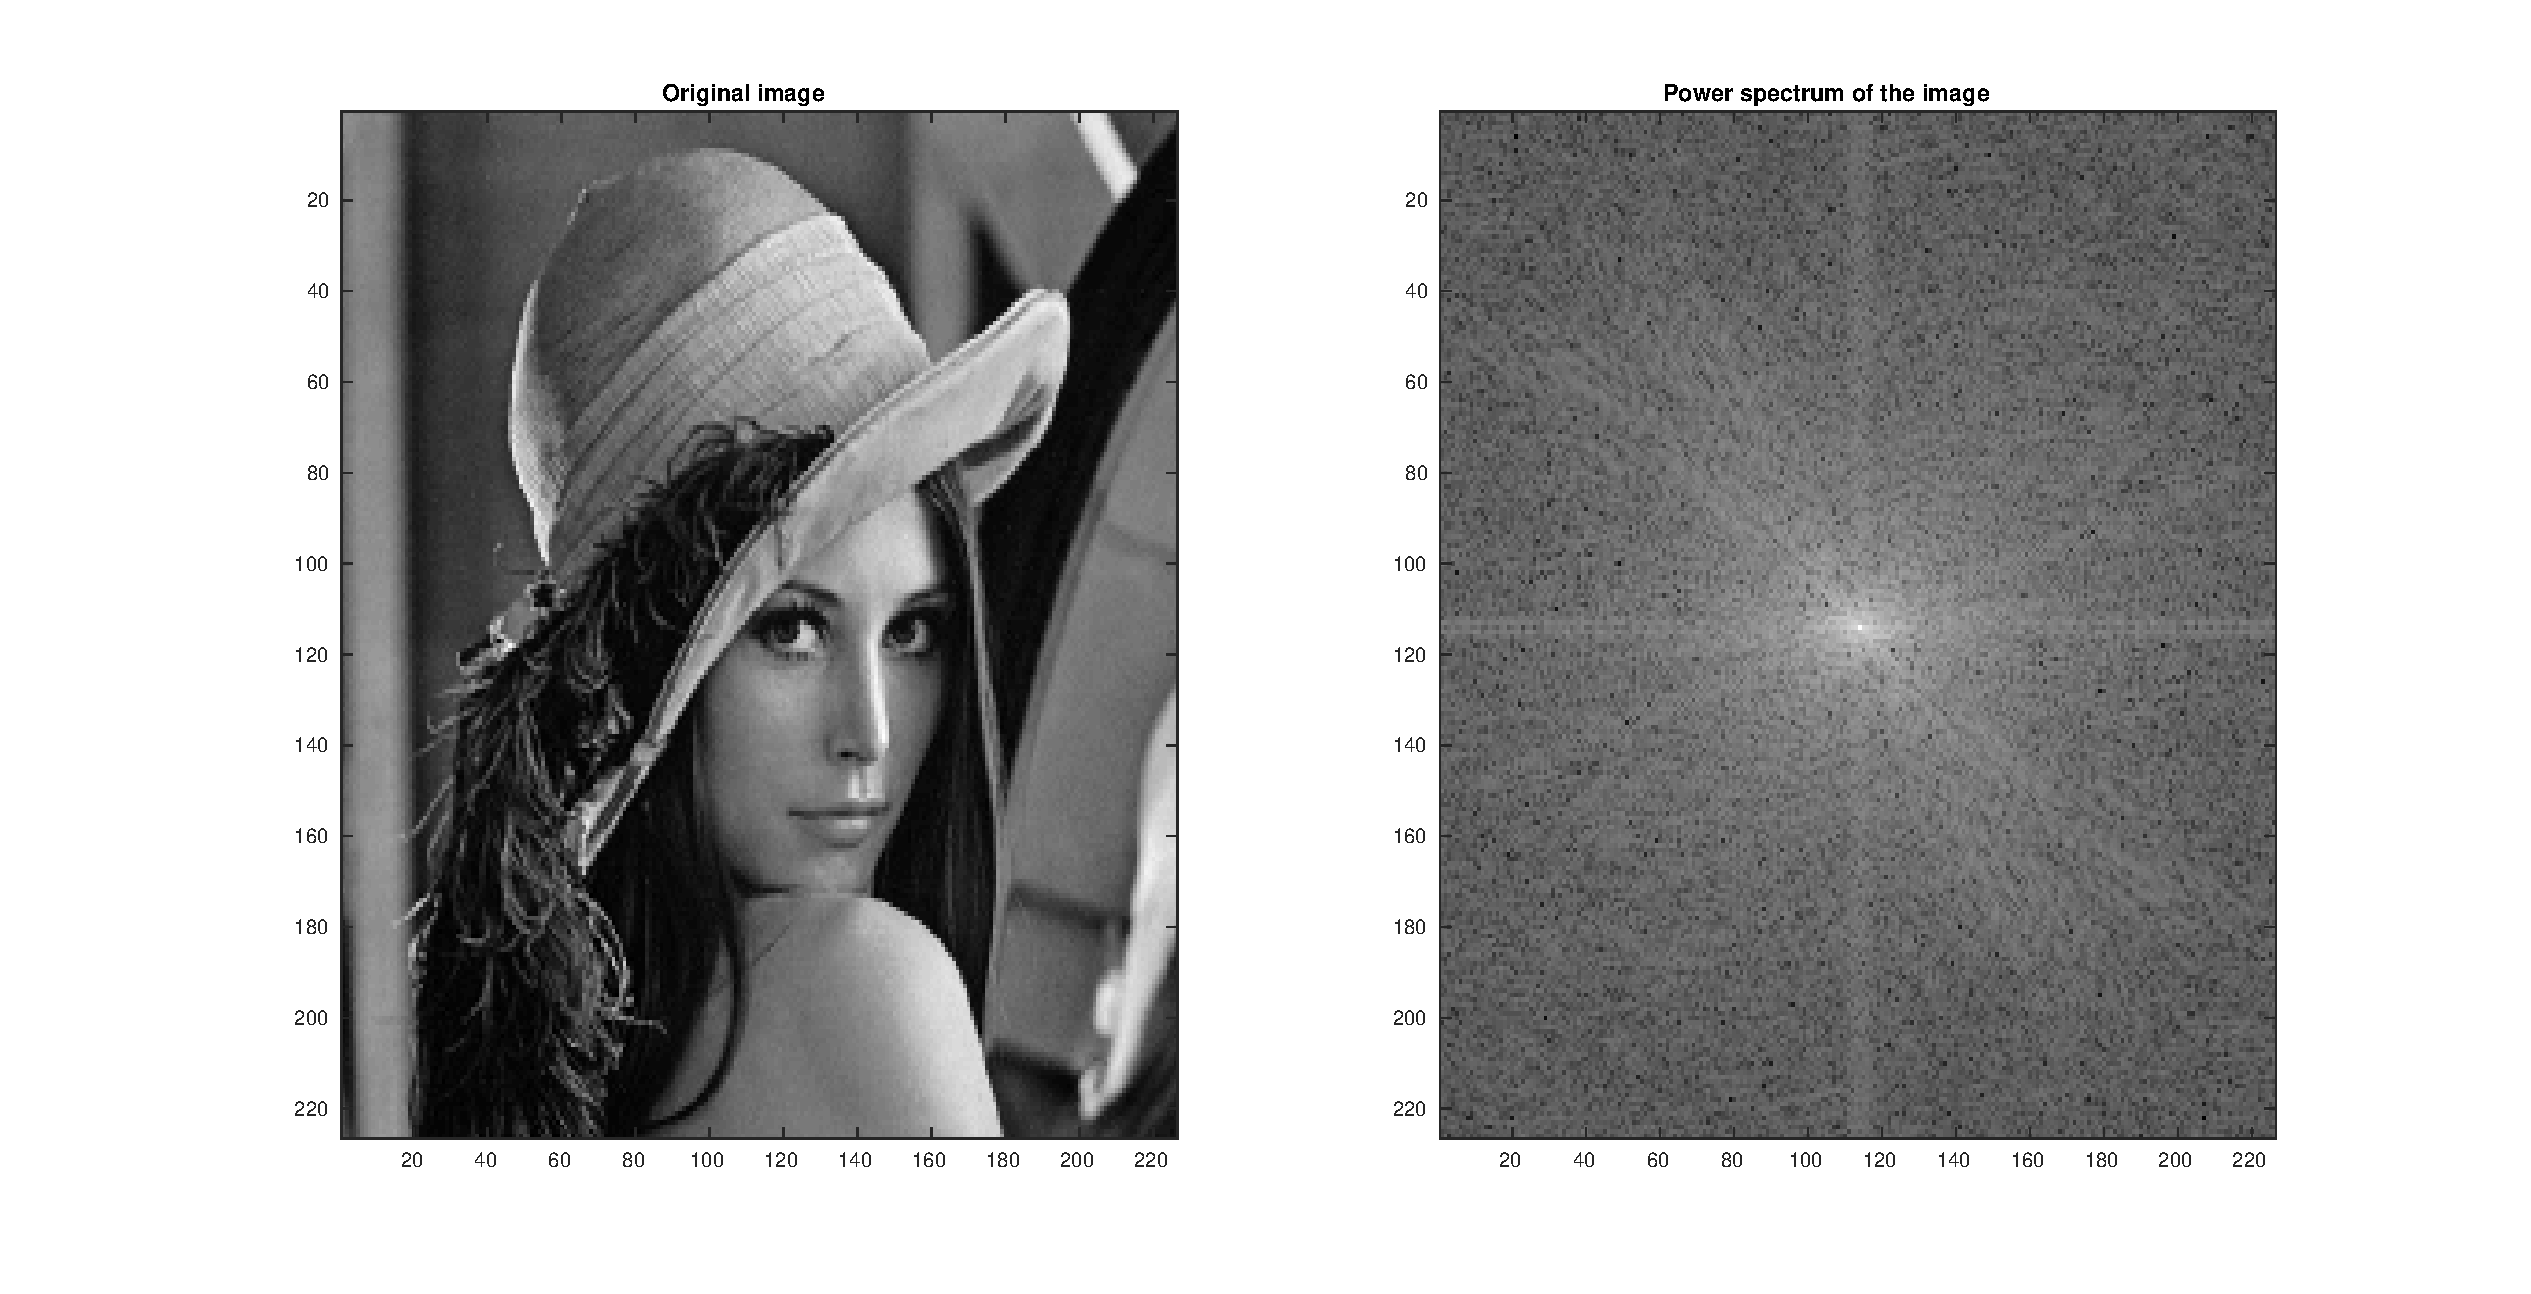
\includegraphics[scale=0.5]{fig1}
  \caption{Graph given by the relation $R$.}
  \label{fig1}
\end{figure}
We see that we can
\begin{itemize}
  \item Reach $1$, $3$, $4$ and $7$ from $1$.
  \item Reach $1$, $3$, $4$ and $7$ from $2$.
  \item Reach nothing from $3$.
  \item Reach $1$, $3$, $4$ and $7$ from $4$.
  \item Reach $1$, $3$, $4$, $6$ and $7$ from $5$
  \item Reach $1$, $3$, $4$, $6$ and $7$ from $6$
  \item Reach $1$, $3$, $4$ and $7$ from $7$.
  \item Reach $1$, $3$, $4$, $6$ and $7$ from $8$.
\end{itemize}
So our transitive closure, $R^+$, is given by:
\begin{align*}
  R^+ &=
  \begin{pmatrix}
    1 & 0 & 1 & 1 & 0 & 0 & 1 & 0 \\
    1 & 0 & 1 & 1 & 0 & 0 & 1 & 0 \\
    0 & 0 & 0 & 0 & 0 & 0 & 0 & 0 \\
    1 & 0 & 1 & 1 & 0 & 0 & 1 & 0 \\
    1 & 0 & 1 & 1 & 0 & 1 & 1 & 0 \\
    1 & 0 & 1 & 1 & 0 & 1 & 1 & 0 \\
    1 & 0 & 1 & 1 & 0 & 0 & 1 & 0 \\
    1 & 0 & 1 & 1 & 0 & 1 & 1 & 0 \\
  \end{pmatrix}
\end{align*}
And the reflexive-transitive closure, $R^*$, is then given by:
\begin{align*}
  R^* &=
  \begin{pmatrix}
    1 & 0 & 1 & 1 & 0 & 0 & 1 & 0 \\
    1 & 1 & 1 & 1 & 0 & 0 & 1 & 0 \\
    0 & 0 & 1 & 0 & 0 & 0 & 0 & 0 \\
    1 & 0 & 1 & 1 & 0 & 0 & 1 & 0 \\
    1 & 0 & 1 & 1 & 1 & 1 & 1 & 0 \\
    1 & 0 & 1 & 1 & 0 & 1 & 1 & 0 \\
    1 & 0 & 1 & 1 & 0 & 0 & 1 & 0 \\
    1 & 0 & 1 & 1 & 0 & 1 & 1 & 1 \\
  \end{pmatrix}
\end{align*}

\subsection{(d)}
The relation $R_1$ is:
\begin{itemize}
  \item Symmetric (since if $|A|\neq |B|$, then obviously $|B|\neq|A|$).
  \item Irreflexive (as $|A| = |A|$)
\end{itemize}
And nothing else. Mostly because it is not transitive as we can have $|A|\neq |B|$ and
$|B|\neq |C|$, but $|A|=|C|$, so it is not any of the orders either. The relation $R_2$ has the
following properties:
\begin{itemize}
  \item Transitive (if $|x|<|y|$ and $|y|<|z|$, then obviously $|x|<|z|$).
  \item Irreflexive (cannot have $|x|<|x|$).
  \item Assymetric (cannot have $|x|<|y|$ and $|y|<|x|$).
  \item Antisymmetric (since it is assymetric).
  \item Strict order (since it is irreflexive and transitive).
  \item Acyclic (since we cannot have $|x|<|y|<|x|$).
\end{itemize}
So it has a few more properties.

\section{Schröder Equivalences and Dedekind Formula}
\subsection{(a)}
TODO

\subsection{(b)}
TODO

\subsection{(c)}
TODO

\subsection{(d)}
TODO

\section{Relational Programming}
\subsection{(a)}
A program computing a tournament of a given relation $R$ can be seen below:
\begin{verbatim}
  Tournament(R)
    DECL S,T,U
    BEG
      S = R & -I(R)
      T = trans(succ(S)) & S
      U = S & -S^
      RETURN T | U
    END.
\end{verbatim}
The first thing we do is to remove $I$ from $R$ as the resulting relation is assymetric.
The resulting relation is stored in $S$. \\
Since we are not computing a completely random tournament of $R$, the idea was to use an
upper triangular matrix without the diagonal (transitive closure of the successor
relation in \textsc{RelView}) and take the intersection with $R$ to set everything below
the diagonal to zero. This would result in a valid tournament of $R$. This is stored in
$T$. \\
However, if we are not expected to be given a symmetric relation $R$, we might want the
edges (that essentially already have a direction) to be in $R$ as well. These edges are
found by taking the intersection of $S$ and $\overline{S^T}$ and are stored in $U$. We
can now take the union of $T$ and $U$ to compute a tournament of any relation $R$. \\
\\
Since the implementation takes the transitive closure to construct the upper triangular
matrix, the running time would depend on the implementation of that. With Warshall's
algorithm, this would give us $\mathcal{O}(n^3)$ for a $n$ by $n$ matrix. However, it is
easy to see that it can be constructed in $\mathcal{O}(n^2)$, where $n$ is the dimension
of $R$ (it is guaranteed to be square as it represents a graph). The intersection and
union are easily computed in $\mathcal{O}(n^2)$ as well. We do a constant amount of these
operation, so the implemented program has time complexity $\mathcal{O}(|V|^2)$, since $n$
is the number of vertices in the graph.\\
\\
Given the relation $R$ defined by:
\begin{figure}[H]
  \centering
  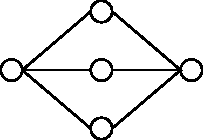
\includegraphics[scale=0.75]{fig3}
  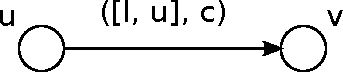
\includegraphics[scale=0.75]{fig6}
  \caption{Relation $R$}
\end{figure}
As a graph, it contains $12$ undirected edges (which are shown as directed in both ways) and
a single directed edge (from nodes $8$ to $7$). The resulting tournament is as both a matrix and a graph is:
\begin{figure}[H]
  \centering
  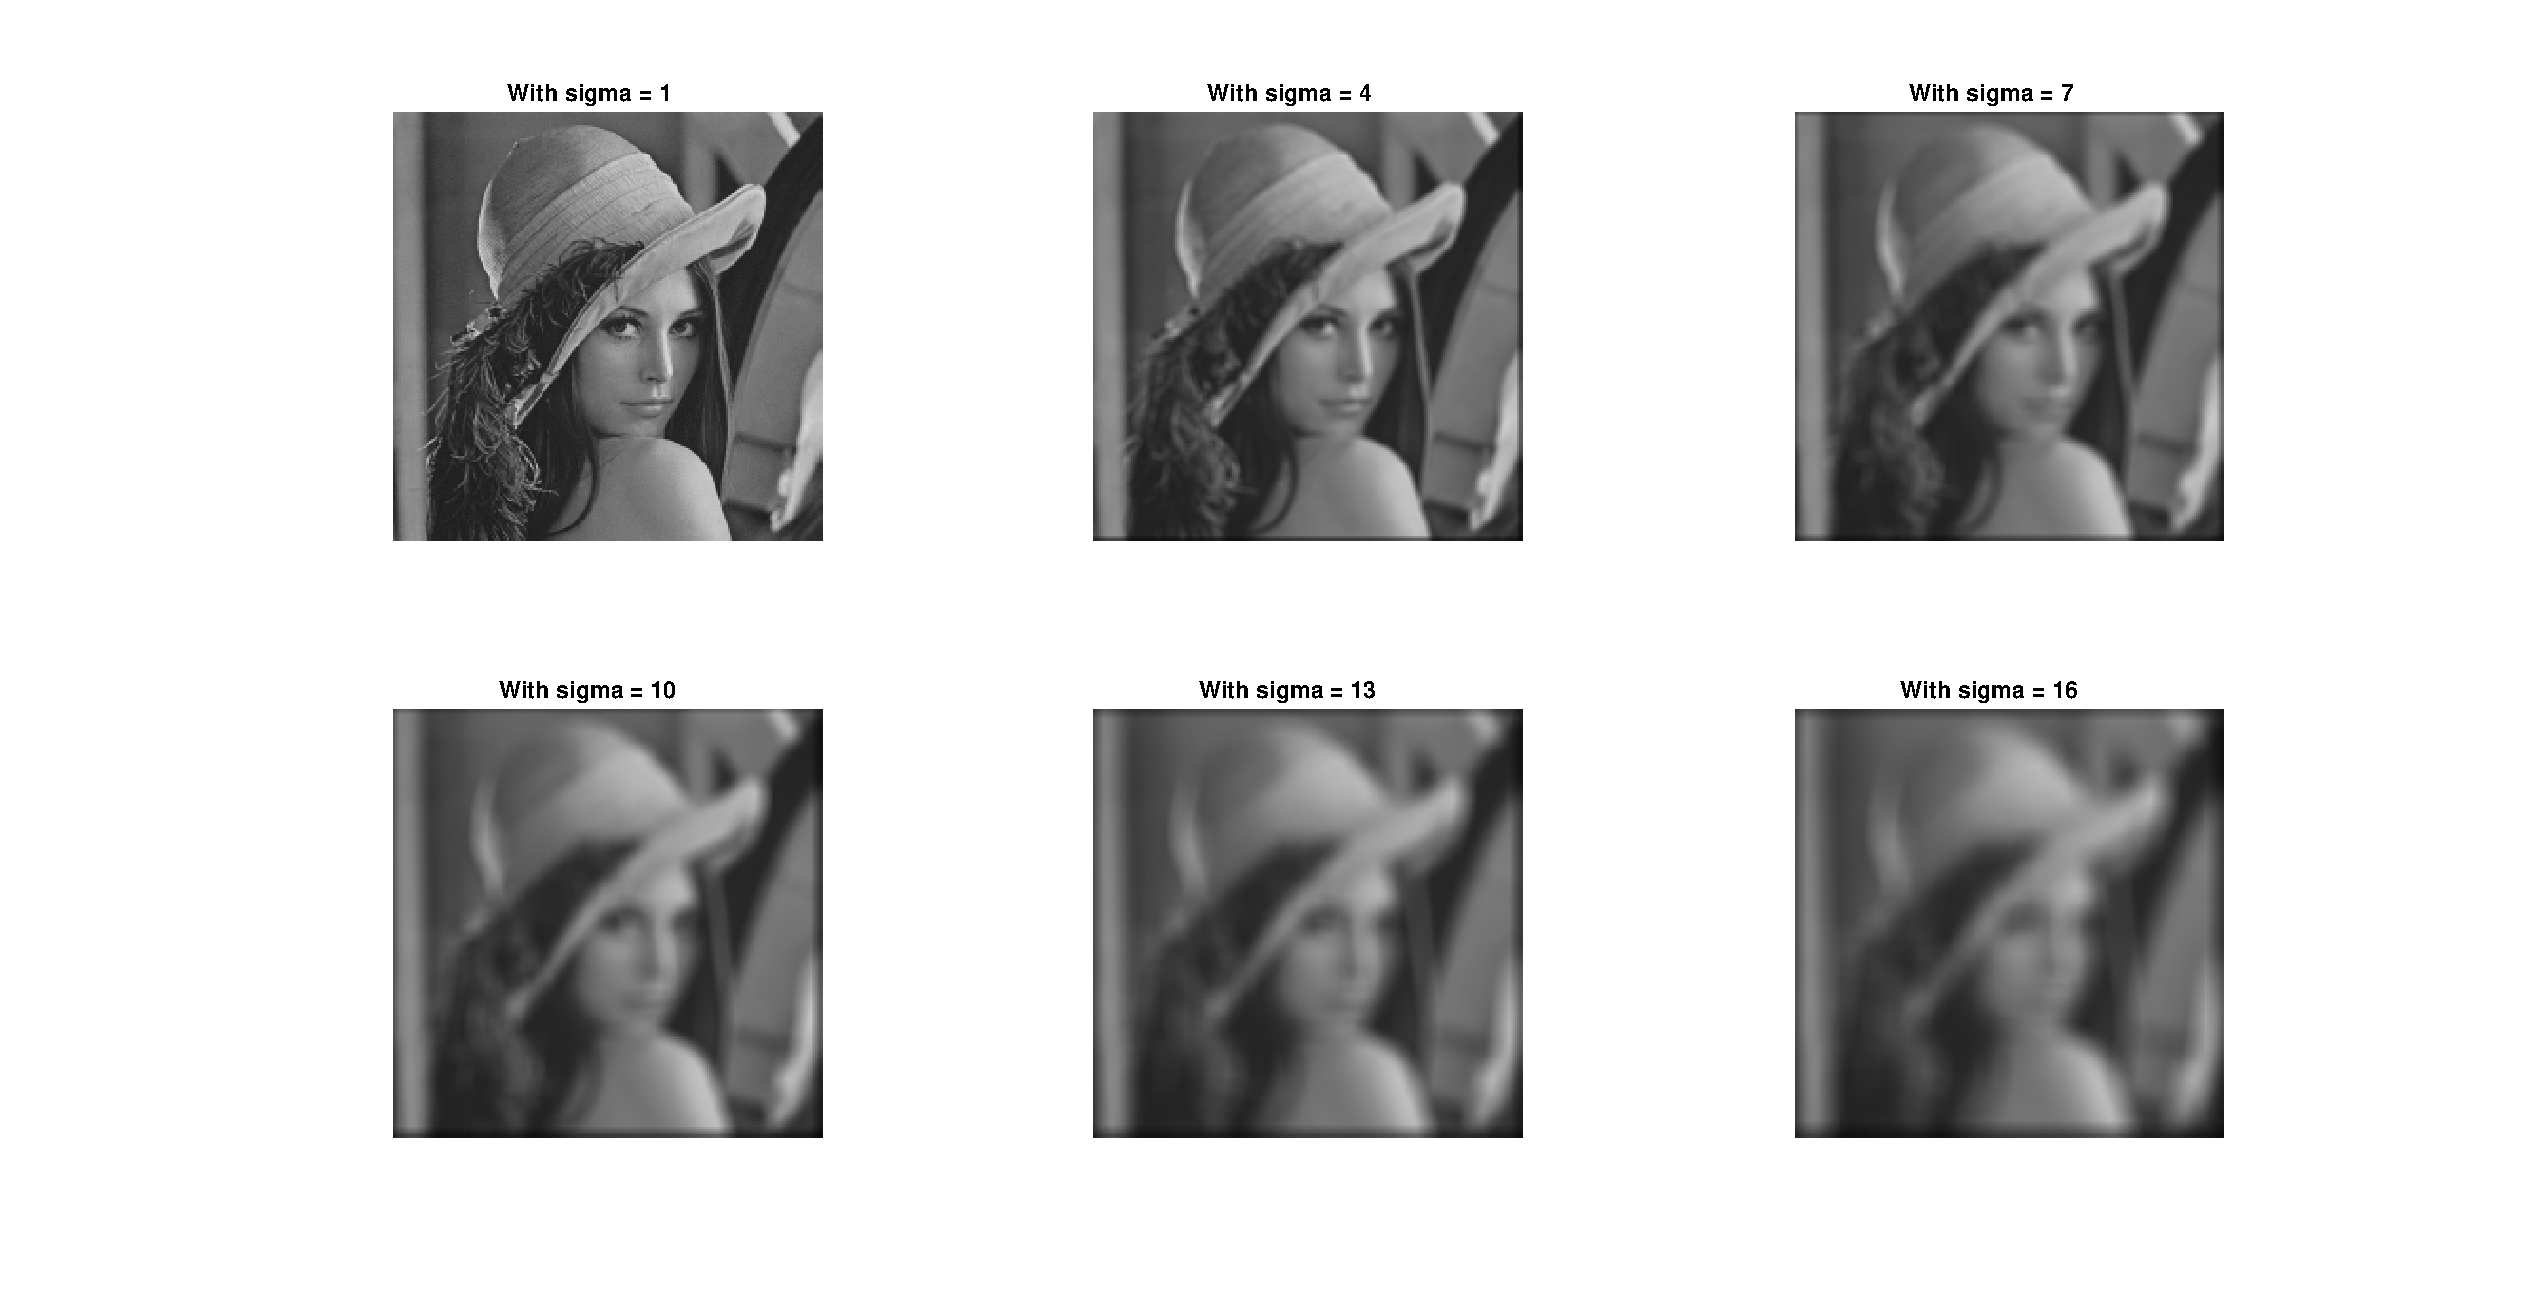
\includegraphics[scale=0.75]{fig4}
  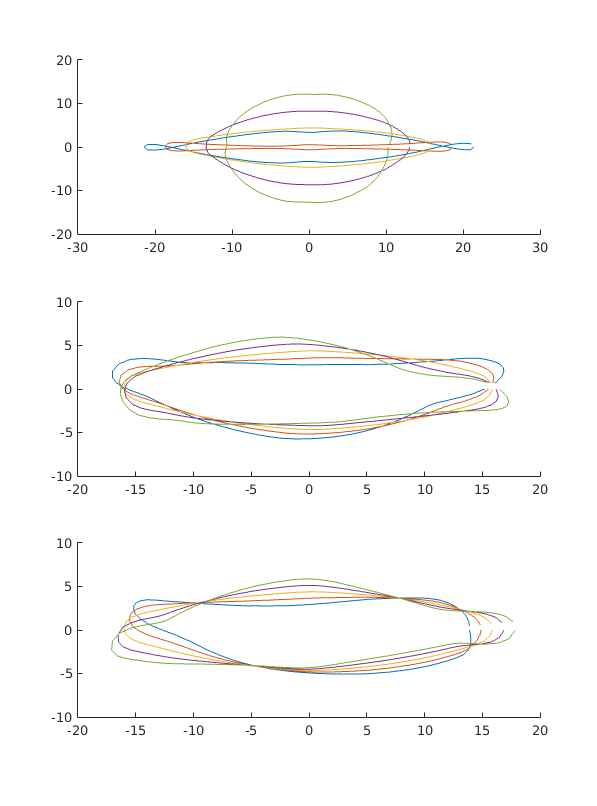
\includegraphics[scale=0.75]{fig5}
  \caption{Result from running the program \texttt{Tournament} on $R$}
\end{figure}
The computed relation is a tournament as all edges have a direction. The result also
contains the edge that was already directed edge. I realize
now that the defintion of the tournament was "an asymmetric relation whose symmetric
closure is $R$", means we probably could have assumed that $R$ is symmetric! One thing to
note is this implementation favors outgoing edges from lower numbered nodes and ingoing
to the higher numbered ones.

\subsection{(b)}
TODO

\subsection{(c)}
The following program check if relation $R$ contains a triangle:
\begin{verbatim}
ContainsTriangle(R)
  DECL S
  BEG
    S = R & -I(R)
    S = S * R
    S = S * R
    RETURN -empty(S & I(R))
  END.
\end{verbatim}
It removes any self loop the relation might have and then computes the composition of
itself twice. Taking composition with itself actually tells us what nodes can be
reached from any node by taking another step in the graph. So if the graph contains a
triangle, a node should be able to reach itself after taking two steps. So if there are
any set entries on the diagonal after the two steps, that means the graph contains a
triangle, which is the test in the return statement. It does not matter if the edges are
directed or not, though the program only detects a triangle if it is a valid path through
the graph.\\
\\
The running time of the program is determined by the time complexity of the computing the
composition of two relations as it dominates the intersection calculations. I believe the
most common way to do this is by matrix multiplication, which with the
Coppersmith–Winograd algorithm can be achieved in $\mathcal{O}(n^{2.376})$, though the
schoolbook algorithm runs in $\mathcal{O}(n^3)$. \\
\\
Consider the following relation, $R$, that does not contain a triangle:
\begin{figure}[H]
  \centering
  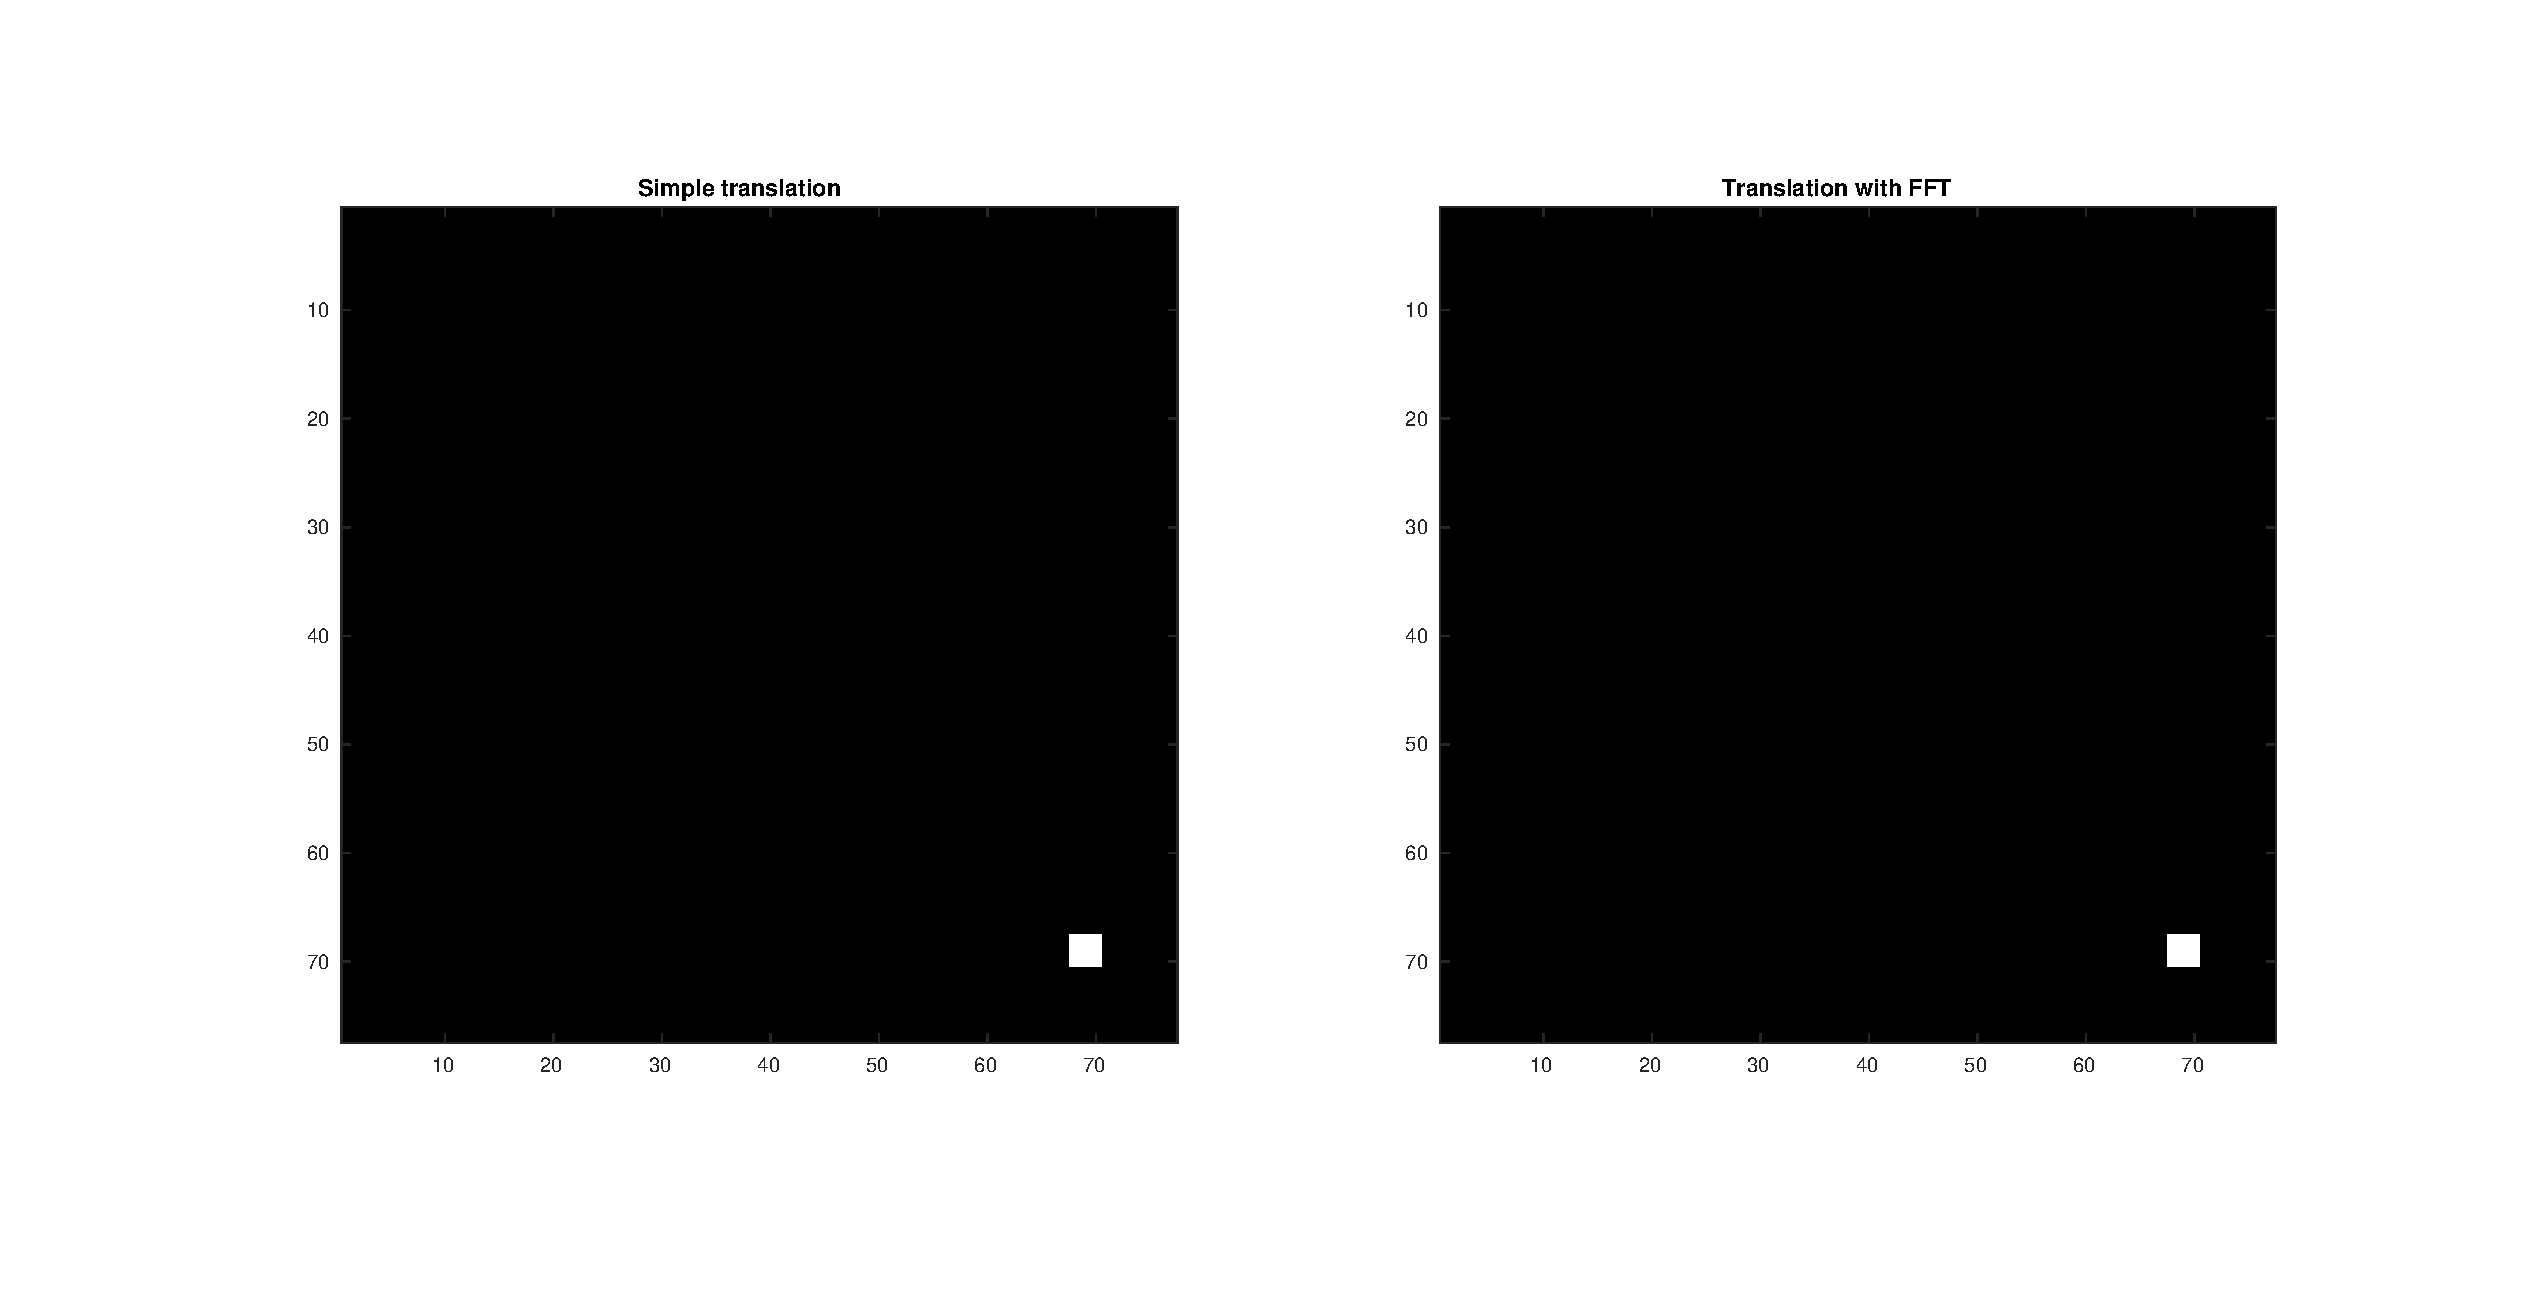
\includegraphics[scale=0.75]{fig7}
  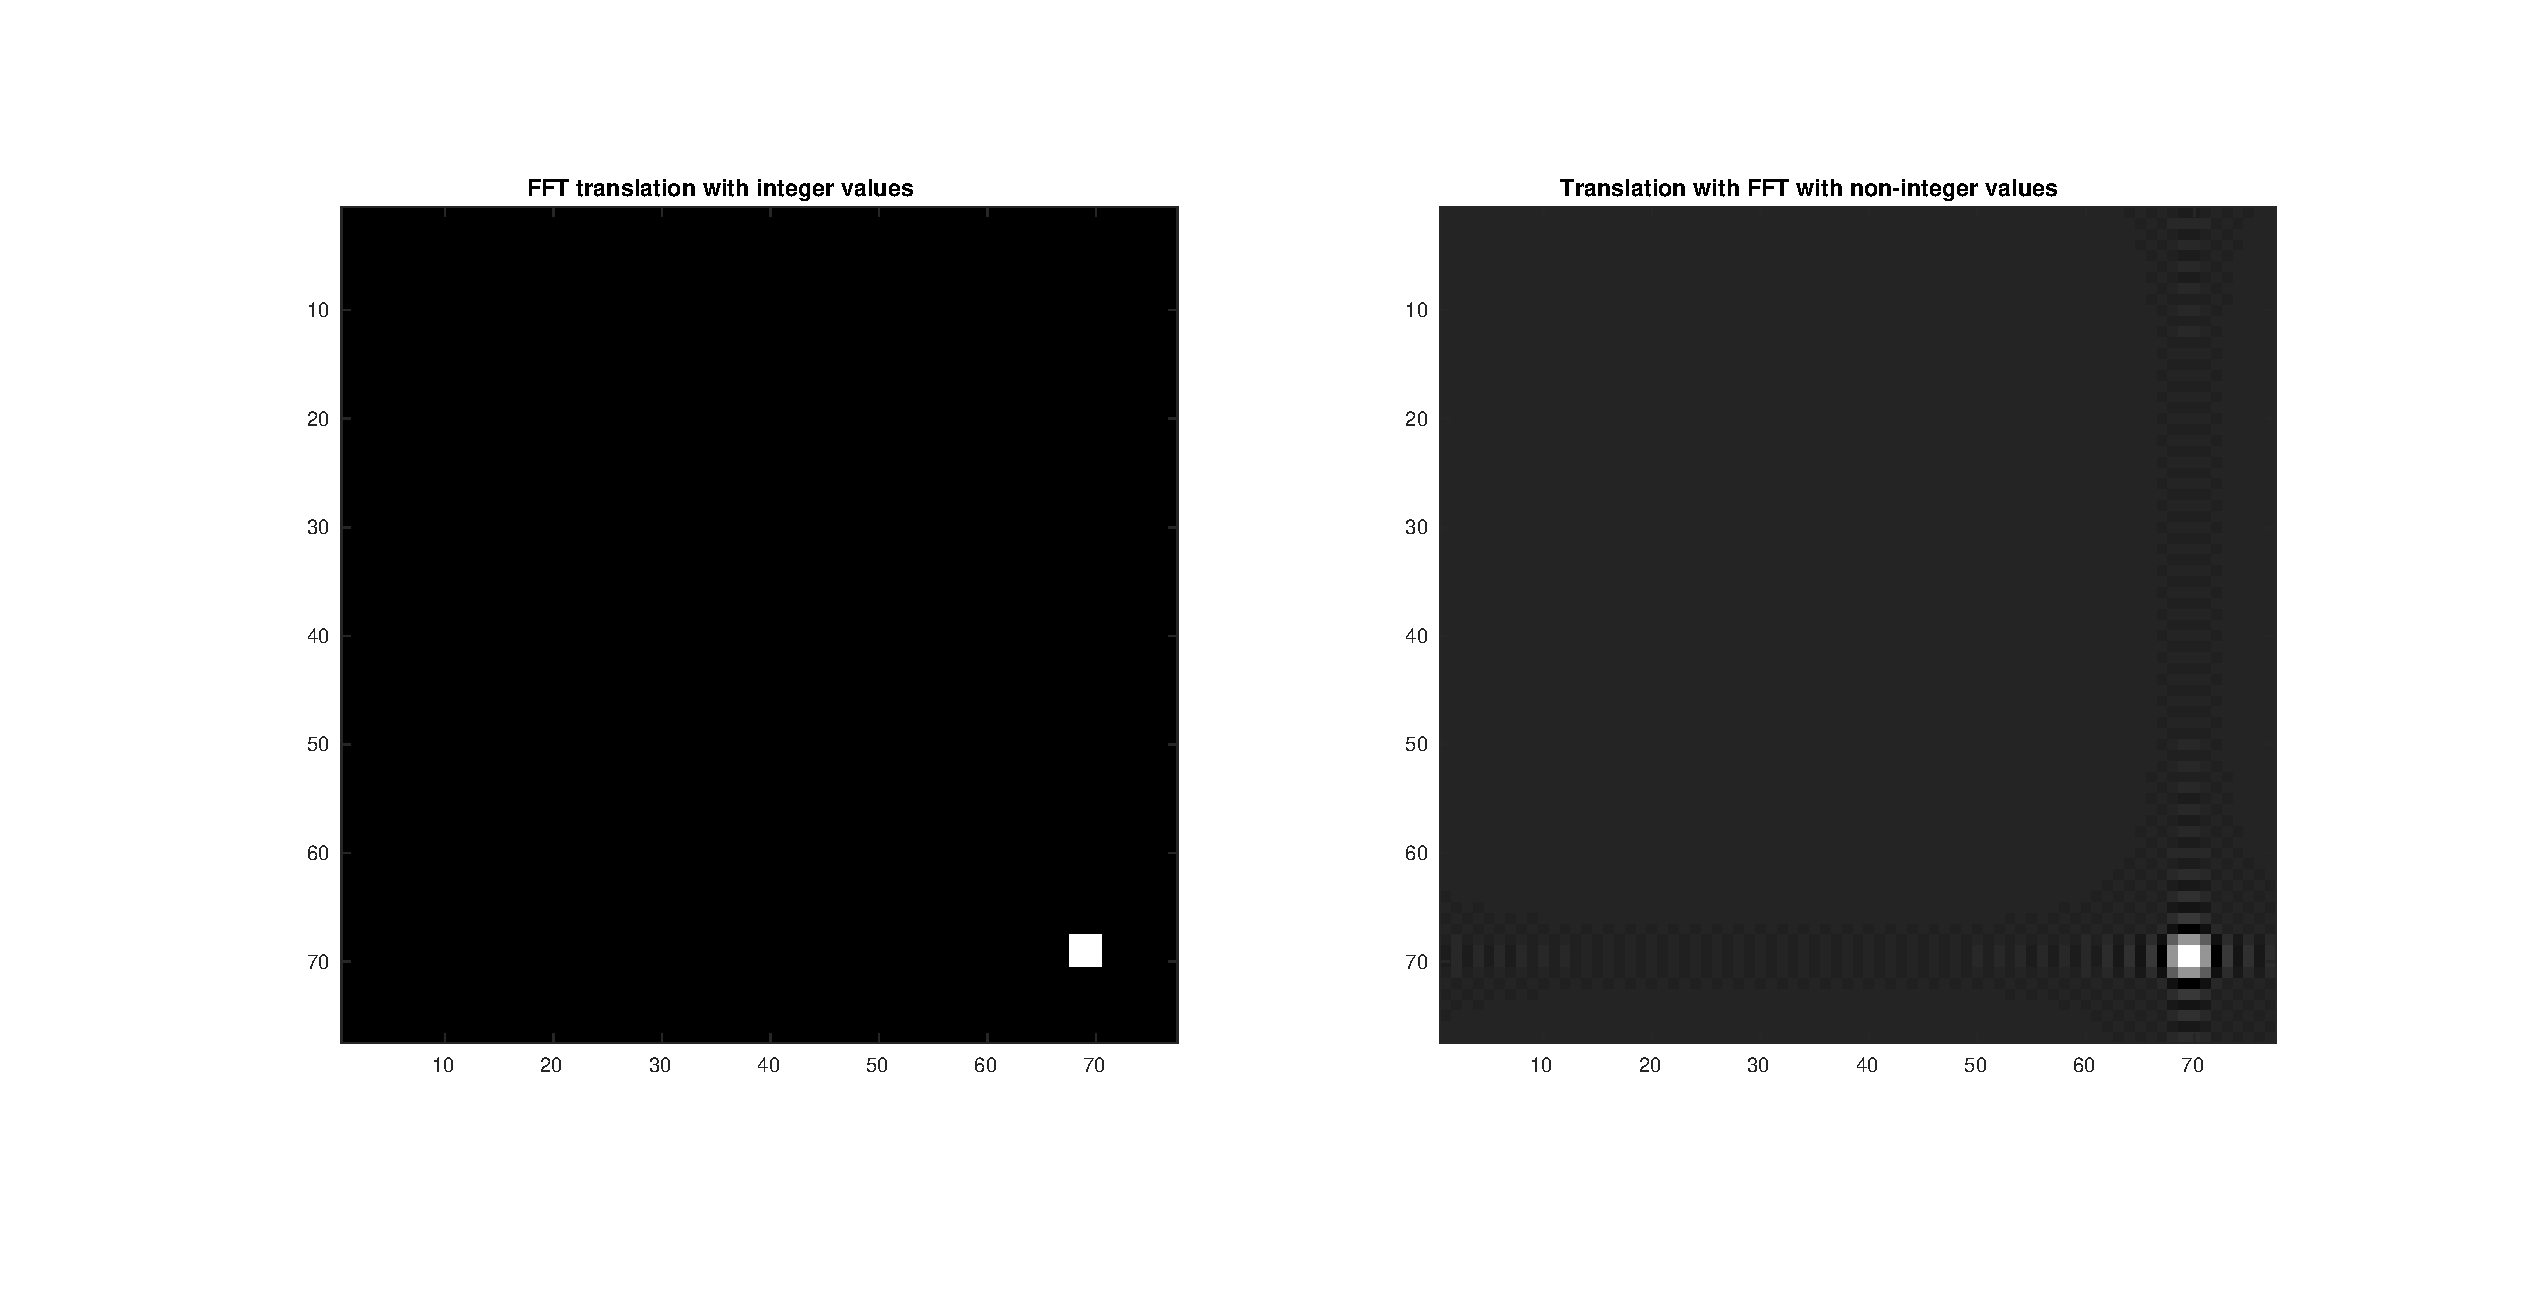
\includegraphics[scale=0.75]{fig8}
  \caption{Relation $R$ which does not contain a triangle.}
\end{figure}
The relation contains no triangles, but does have a cycle of size $2$, $4$, $5$, $6$, $7$
and $8$. Note that $\{2,3,6\}$ is not a triangle as both edges out of $6$ are outgoing.
The program outputs a single cell which is empty (contains no triangle). We can change
relation $R$ to $R'$ by adding a direction from $3$ to $6$ giving us:
\begin{figure}[H]
  \centering
  \includegraphics[scale=0.75]{fig9}
  \includegraphics[scale=0.75]{fig10}
  \caption{Relation $R'$ which contains the triangle consisting of node $2$, $3$ and $6$.}
\end{figure}
Running the program now outputs a single non-empty cell since there exist a triangle in the
vertex set $\{2,3,6\}$.

\section{Modelling}
\subsection{(a)}
Since $D$ is a partial order, it is reflexive (it divides itself), meaning $I\subseteq
D$. Since $IL=LI=L$, we must have that $LD=L=DL$.

\subsection{(b)}
One way to represent a subset is by a vector. We define the set $E$ as:
\begin{align*}
  E = \overline{\overline{D}L}
\end{align*}
as $1$ is the only element that divides every other element, so row $1$ in $\overline{D}$
will have all zeroes as the only row, meaning it is the only row containing zeroes in
$\overline{D}L$ and therefore the only one to contain $1$'s in $\overline{\overline{D}L}$.

\subsection{(c)}
\subsubsection{(i)}
We want to prove that:
\begin{align*}
  E &= \overline{\overline{D}L} \\
    &\subseteq D
\end{align*}
This holds iff:
\begin{align*}
  \overline{D}&\subseteq \overline{\overline{\overline{D}L}}
  \comment{$\overline{\phantom{I}}$ is
$\subseteq$-antitone} \\
&=\overline{D}L \comment{$\overline{\phantom{I}}$ is involutive}
\end{align*}
which holds since composition with $L$ from the right is $\subseteq$-increasing.

\subsubsection{(ii)}
Remember that $E$ is a vector iff $E=EL$, so we have:
\begin{align*}
  E&=\overline{\overline{D}L} \\
   &=
\end{align*}

\subsubsection{(iii)}
\subsubsection{(iv)}
\subsubsection{(v)}

\subsection{(d)}
A prime is a number only divisible by itself and $1$. So one way to way represent the set
$Q$ is by:
\begin{align*}
  Q &= \overline{L\left(D\cap \left(\overline{E}\cap \overline{I}\right)\right)}^T
\end{align*}
To see this, consider the intersection $\overline{E}\cap \overline{I}$. It has $1$ in all
entries, but the ones that were $1$ in $E$ and $I$. Taking the intersection of this with
$D$, gives us $D-E-I$ as we wanted. Now all columns that are all zeroes are the primes
(and $1$), so taking the composition with $L$ from left will fill all other columns with
$1$'s. If we take the complement, all columns in $Q$ are ones instead, and finally we transpose it to represent the set as a row vector as we did with $E$.

\subsection{(e)}
TODO

\subsection{(f)}
For $P$, we just need to remove the element $1$ from $Q$. That is we want $Q-E$, so we
define $P$ as:
\begin{align*}
  P&=Q\cap \overline{E}
\end{align*}
Since $E\subset Q$, we can just take the intersection of $Q$  and the complement of $E$
and we are left with the elements in $Q$ that were not in $E$.

\end{document}
